%% Based on a TeXnicCenter-Template by Gyorgy SZEIDL.
%%%%%%%%%%%%%%%%%%%%%%%%%%%%%%%%%%%%%%%%%%%%%%%%%%%%%%%%%%%%%

%------------------------------------------------------------
%
%\documentclass{article}%
%Options -- Point size:  10pt (default), 11pt, 12pt
%        -- Paper size:  letterpaper (default), a4paper, a5paper, b5paper
%                        legalpaper, executivepaper
%        -- Orientation  (portrait is the default)
%                        landscape
%        -- Print size:  oneside (default), twoside
%        -- Quality      final(default), draft
%        -- Title page   notitlepage, titlepage(default)
%        -- Columns      onecolumn(default), twocolumn
%        -- Equation numbering (equation numbers on the right is the default)
%                        leqno
%        -- Displayed equations (centered is the default)
%                        fleqn (equations start at the same distance from the right side)
%        -- Open bibliography style (closed is the default)
%                        openbib
% For instance the command
\documentclass[a4paper]{article}
%           \documentclass[final,narroweqnarray,inline]{ieee}
% ensures that the paper size is a4, the fonts are typeset at the size 12p
% and the equation numbers are on the left side

%------------------------------------------------------------

%%%%%%%%%%%%%%%%%%%%%%%%%%%%%%%%%%%%%%%%%%%%%%%%%%%%%%%%%%%%%
%Basic Latex Einf\UTF{00B8}hrung
%http://www.thomastaubert.de/htm/latex.htm
%http://www.uni-koeln.de/rrzk/kurse/unterlagen/latex/ergaenzungen/pdftex.pdf
%%%%%%%%%%%%%%%%%%%%%%%%%%%%%%%%%%%%%%%%%%%%%%%%%%%%%%%%%%%%%

%------------------------------------------------------------

%------------------------------------------------------------

%%%%%%%%%%%%%%%%%%%%%%%%%%%%%%%%%%%%%%%%%%%%%%%%%%%%%%%%%%%%%
\usepackage{amsmath}
\usepackage{amsfonts}
\usepackage{amssymb}
\usepackage[ngerman]{babel}


% umlaute
\usepackage[utf8]{inputenc}
%\usepackage{ngerman}


%Package for figures
\usepackage{graphicx}
\usepackage{subfigure}
%Caption: kleinere Schriftgr\UTF{00F6}sse f\UTF{00FC}r die Bildbeschreibung
\usepackage[hang,nooneline,footnotesize,bf]{caption}

%Package for formating SI Units
\usepackage{sistyle}

%Package um die Zitate zu sortieren 
%Anstelle von "`ich zitiere hier \cite[a],\cite[b] und \cite[c]"'
%einfach nur schreiben "`ich zitiere hier \cite[a,b,c]"' 
\usepackage{cite}

%Zum \UTF{00B8}berladen von LaTex Befehlen
\usepackage{ifthen}

%Package f\UTF{00B8}r Source-Code Darstellung
\usepackage{listings}

% Longtable: \UTF{00B8}berlange Tabellen automatisch umbrechen
\usepackage{longtable}

% this is for layout testing
\usepackage{layout}

% Packag Hyperref erlaubt die Eigenschaften und links von PDFs zu aktivieren
% Look at http://en.wikibooks.org/wiki/LaTeX/Packages/Hyperref
\usepackage[pdftex]{hyperref}
\hypersetup{
    %bookmarks=true,         % show bookmarks bar?
    unicode=true,          % non-Latin characters in Acrobat\UTF{00ED}s bookmarks
    pdftoolbar=true,        % show Acrobat\UTF{00ED}s toolbar?
    pdfmenubar=true,        % show Acrobat\UTF{00ED}s menu?
    pdffitwindow=true,      % page fit to window when opened
    pdftitle={Multi Modal Logiken},    % title
    pdfauthor={Waldemar Schwan},     % author
    pdfsubject={},   % subject of the document
    pdfnewwindow=true,      % links in new window
    pdfkeywords={multi modal logics}, % list of keywords
    colorlinks=true,       % false: boxed links; true: colored links
    linkcolor=black,          % color of internal links
    citecolor=black,        % color of links to bibliography
    filecolor=black,      % color of file links
    urlcolor=black,           % color of external links
    hypertexnames=false	% solves Problems with Links
}


%%%%%%%%%%%%%%%%%%%%%%%%%%%%%%%%%%%%%%%%%%%%%%%%%%%%%%%%%%%%%
%Shortcuts f\UTF{00B8}r Copyright, Trademark und Registered
\def\TReg{\textsuperscript{\textregistered}} %use \TReg for Registered
\def\TCop{\textsuperscript{\textcopyright}}  %use \TCop for Copyright
\def\TTra{\textsuperscript{\texttrademark}}  %use \TTra for Trademark


%% Nummerierung der \UTF{00DC}erschriften
%\renewcommand \thechapter {\Roman{chapter}.}
%\renewcommand \thesection {\Alph{section})}
%\renewcommand \thesubsection {\arabic{subsection}.}
%\renewcommand \thesubsubsection {\alph{subsubsection})}
%\renewcommand \theparagraph {}     % oder: {(\arabic{paragraph})}
%%Alternative: Paket "alnumsec" / s.u.


% erstellt eine Fu\UTF{FB02}note mit Vgl. und dahinter die zitierte Stelle
% \vgl{Quelle05} -> vgl. Quelle 2005
% \vgl[S. 123]{Quelle05} -> vgl. Quelle 2005, S. 123

%
% erstellt eine Fu\UTF{FB02}note mit der zitierten Stelle
% \zitat{Quelle05} -> Quelle 2005
% \zitat[S. 123]{Quelle05} -> Quelle 2005, S. 123
\newcommand{\zitat}[2][]{\footnote{\cite{#2}\ifthenelse{\equal{#1}{}}{}{, #1}}}

%f\UTF{00B8}gt eine Fu\UTF{FB02}note mit Verweis und Seitenzahl des angegebenen Label ein.
\newcommand{\vglFuss}[1]{\footnote{vgl. Kapitel \ref{#1} auf Seite \pageref{#1}}}

%Erlaubt r\UTF{00F6}mische Ziffern zu nutzen
\newcommand{\RMDOT}[1]{\MakeUppercase{\romannumeral #1{.}}}
\newcommand{\RM}[1]{\MakeUppercase{\romannumeral #1}}
%%%%%%%%%%%%%%%%%%%%%%%%%%%%%%%%%%%%%%%%%%%%%%%%%%%%%%%%%%%%%

%------------------------------------------------------------

\usepackage{dsfont}
%!TEX root = /Users/velrok/Dropbox/TheoInf Seminar/Ausarbeitung/Main.tex

%email format
\newcommand{\emailAdress}[1]{\textless\href{mailto:#1}{#1}\textgreater}


% für notizen
\usepackage{color}
\newcommand{\todo}[1]{\textcolor{red}{\textless\textbf{#1}\textgreater}}

%------------------------------------------------------------

%%%%%%%%%%%%%%%%%%%%%%%%%%%%%%%%%%%%%%%%%%%%%%%%%%%%%%%%%%%%%
\newtheorem{theorem}{Theorem}
\newtheorem{acknowledgement}[theorem]{Acknowledgement}
\newtheorem{algorithm}[theorem]{Algorithm}
\newtheorem{axiom}[theorem]{Axiom}
\newtheorem{case}[theorem]{Case}
\newtheorem{claim}[theorem]{Claim}
\newtheorem{conclusion}[theorem]{Conclusion}
\newtheorem{condition}[theorem]{Condition}
\newtheorem{conjecture}[theorem]{Conjecture}
\newtheorem{corollary}[theorem]{Corollary}
\newtheorem{criterion}[theorem]{Criterion}
\newtheorem{definition}[theorem]{Definition}
\newtheorem{example}[theorem]{Example}
\newtheorem{exercise}[theorem]{Exercise}
\newtheorem{lemma}[theorem]{Lemma}
\newtheorem{notation}[theorem]{Notation}
\newtheorem{problem}[theorem]{Problem}
\newtheorem{proposition}[theorem]{Proposition}
\newtheorem{remark}[theorem]{Remark}
\newtheorem{solution}[theorem]{Solution}
\newtheorem{summary}[theorem]{Summary}
\newenvironment{proof}[1][Proof]{\textbf{#1.} }{\ \rule{0.5em}{0.5em}}
%%%%%%%%%%%%%%%%%%%%%%%%%%%%%%%%%%%%%%%%%%%%%%%%%%%%%%%%%%%%%

%------------------------------------------------------------

%BEGIN DES EIGENTLICHEN DOKUMENTES

%------------------------------------------------------------

%%%%%%%%%%%%%%%%%%%%%%%%%%%%%%%%%%%%%%%%%%%%%%%%%%%%%%%%%%%%%

\title{Multi Modal Logiken}
\author{Waldemar Schwan}

\begin{document}
	
%!TEX root = /Users/velrok/Dropbox/TheoInf Seminar/Ausarbeitung/Main.tex

\begin{titlepage}
	
	\vspace*{0.8cm}
	
	\begin{center}
		\begin{Huge}
			\MMLn
		\end{Huge}
	\end{center}
	
	\vspace*{2cm}
	
	\begin{center}
		\begin{Large}
			Seminar Theoretische Informatik\\
			Hochschule Bonn-Rhein-Sieg\\
			SS 2011
		\end{Large}			
	\end{center}

	\vspace*{3.5cm}
	
	\begin{center}
		\begin{Large}
			Waldemar Schwan \emailAdress{waldemar.schwan@smail.inf.h-brs.de}
		\end{Large}			
	\end{center}
	%
	\vspace*{4.5cm}
	%
	\begin{large}
		Betreuer: Prof. Dr. Martin Eric Müller \emailAdress{martin.mueller@h-brs.de}\\
		Betreuer: Prof. Dr. Alexander Asteroth \emailAdress{alexander.asteroth@h-brs.de}\\
	\end{large}
	%
	\\
	Stand: \today
\end{titlepage}
	
	
	
%\layout
%\include{Titelseite}
%	\renewcommand{\baselinestretch}{1.1}\normalsize

\tableofcontents
\newpage

%\listoftables
%\listoffigures
%\newpage


%!TEX root = /Users/velrok/Dropbox/TheoInf Seminar/Ausarbeitung/Main.tex

%!TEX root = /Users/velrok/Dropbox/TheoInf Seminar/Ausarbeitung/Main.tex

\section{Eigenschaften, Anwendungsfelder} % (fold)
\label{sec:eigenschaften_anwendungsfelder}

\paragraph{Wahrheits-Modi} % (fold)
\label{par:wahrheits_modi}

Die Aussagenlogik und Prädikatenlogik kennen nur eine Art von Wahr oder Falsch. Im realen Leben unterscheiden wir jedoch ganz intuitiv zwischen einer Vielzahl von unterschiedlichen Wahrheiten.
Die Aussage \emph{"Frau Merkel ist die Bundeskanzlerin der BRD"} ist \textbf{im Moment} wahr es kann sich jedoch bei der nächsten Wahl ändern.
Die Aussage \emph{"Die Erde hat einen Mond"} ist jetzt wahr und wird mit an Sicherheit grenzender Wahrscheinlichkeit auch in Zukunft wahr sein. 
Sie ist aber nicht notwendiger Weise Wahr, denn es hätten ja auch 2 oder 3 Monde sein können.
Ein Beispiel für eine notwendigerweise wahre Aussage ist \emph{''ein Junggeselle ist unverheiratet''}. Wir können uns keinen verheirateten Junggestellen vorstellen.\todo{Zitat einfügen}

% paragraph wahrheits_modi (end)

\paragraph{Anwendungsfelder} % (fold)
\label{par:anwendungsfelder}

In der Informatik ist das Schlussfolgern über verschiedene Arten der Wahrheit nützlich in Bereichen wie \emph{Model Checking} und \emph{AI (Artificial Intelligence)}. \\
Im Model Checking kommen vor allem Temporal Logiken zum Einsatz, um Wahrheitsaussagen zu unterschiedlichen Zeiten im Programmablauf treffen zu können. \\
Im Bereich der AI, werden Multi-Modal-Logiken in Multi-Agent-Systemen verwendet. 
Solche Systeme sind in der Lage Schlussfolgerungen, nicht nur aus dem eigenen Wissen, sondern auch aus dem Wissen über das Wissen anderer und deren Wissen zu ziehen.\\
Einfache Logiken modellieren nur eine Modularität von Wahrheit, z.B. notwendigerweise wahr, komplizierte Logiken modellieren auch mehrere, z.B. wahr nach allem was Agent $i$ weis, für $ 0 < i < k$. \cite[S.306f]{huth2004logic}\\

% paragraph anwendungsfelder (end)

\paragraph{Struktur der Arbeit} % (fold)
\label{par:struktur_der_arbeit}

Diese Arbeit ist in zwei Bestandteile aufgeteilt. 

Kapitel \ref{sec:modal_logic} beschäftigt sich mit dem Grundlagen von Modal-Logiken. 
Es erklärt Syntax, Semantik die Modellierung in Form von Kripke-Struckturen und die possible Word Semantik. \todo{stimmt das so?}
Es werden wichtige Eigenschaften von Modal-Logiken aufgeführt und erklärt, sowie der Zusammenhang zwischen der Relation $R$ im Kipke-Model und den vorher beschriebenen Eigenschaften verdeutlicht, bekannt als \emph{Ähnlichkeitstheorie}.
Am Ende wird das Thema anhand der Modal-Logik $KT45$ (für Wissen) konkretisiert.

Kapitel \ref{sec:multi_modal_logic} erklärt Multi-Modal-Logiken, als Modal-Logiken die mehr als nur eine Modalität vereinen. Das Kapitel beginnt mit der Darstellung der \emph{the wise men} und \emph{muddy children} Rätsel. 
Anhand dieser Beispiele wird die Verallgemeinerung der Modal-Logik $KT45$ verdeutlicht und zur Anwendung gebracht um diese Rätsel formal zu lösen.
Im Zuge dieser Lösung wird genauer auf die Multi-Modal-Logik $KT45^n$ eingegangen und deren Unterschiede und Erweiterungen im Vergleich zur Logik $KT45$ erklärt.




% paragraph struktur_der_arbeit (end)

% section eigenschaften_abgrenzung_zur_aussagenlogik (end)

%!TEX root = /Users/velrok/Dropbox/TheoInf Seminar/Ausarbeitung/Main.tex


\chapter{Modal-Logik ($K$)} % (fold)
\label{sec:modal_logic}

%!TEX root = /Users/velrok/Dropbox/TheoInf Seminar/Ausarbeitung/Main.tex

\section{Syntax} % (fold)
\label{sec:syntax}
Die Syntax der Modal Logik entspricht der der Aussagenlogik mit den Erweiterungen $\square$ und $\Diamond$. 
Wie die Negation sind diese unär, das heißt sie beziehen sich nur auf die ihr folgende Formel. Im Folgenden werden die Zeichen $p, q, r, p_3$ für atomare Formeln verwendet.\cite[S.307f]{huth2004logic}\\
\\
\begin{definition}
	\label{def:syntax}
	Die folgende BNF (Backus Naur Form) beschreibt die Syntax der möglichen multi modal Formeln $\phi$.

	\begin{equation}
		\label{eqn:bnf}
		\phi ::= \bot|\top|p|(\neg\phi)|(\phi\wedge\phi)|(\phi\vee\phi)|(\phi\rightarrow\phi)|
		(\phi\leftrightarrow\phi)|(\square\phi)|(\Diamond\phi)
	\end{equation}
\end{definition}
\cite[S.307]{huth2004logic}
\\
\\
Die Formeln 
\begin{equation}
	(p \wedge \Diamond(p \rightarrow \square \neg r))
\end{equation} 
und 
\begin{equation}
	\square((\Diamond q \wedge \neg r) \rightarrow \square p )	
\end{equation}
sind Beispiele für syntaktisch korrekte Multi-Modal-Logik Formeln. Ihre Parse-Trees sind abgebildet in Abbildung~\ref{fig:mmFormel01}.
Wie auch bei der Aussagenlogik binden die unären Operatoren stärker als die Binären.
Sodass unnötige Klammern weggelassen werden können um die Leserlichkeit zu verbessern.\\
\\
\begin{figure}[h!]
	\begin{center}
  	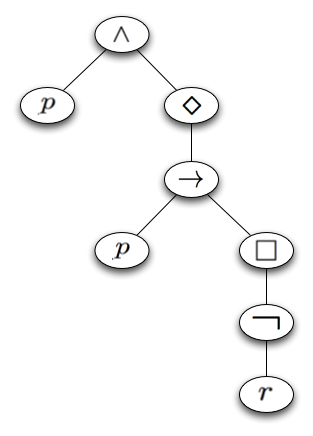
\includegraphics[width=0.4\textwidth]{./Images/mmFormel01.png}
		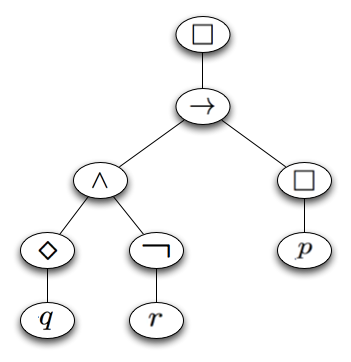
\includegraphics[width=0.4\textwidth]{./Images/mmFormel02.png}
  	\caption{Parse-Tree für $(p \wedge \Diamond(p \rightarrow \square \neg r))$ und 
		$\square((\Diamond q \wedge \neg r) \rightarrow \square p )$}
		\label{fig:mmFormel01}
	\end{center}
\end{figure}
%
Die folgende Liste sortieren die Operatoren nach ihrer Bindungsstärke. 
Beginnend mit den am stärksten bindenden.\\
\begin{itemize}
	\item $\neg, \square, \Diamond$
	\item $\wedge, \vee$
	\item $\rightarrow, \leftrightarrow$
\end{itemize}
%
Im allgemeinen werden die Symbole $\square$ und $\Diamond$ als Box und Raute gelesen. 
Spezifiziert man eine konkrete Logik so werden diese entsprechend ihrer interpretation gelesen. In der Logik für Notwendigkeit wird $\square$ als notwendig und $\Diamond$ als möglich gelesen. In Logik für über das Wissen eines Agenten Q, wird $\square$ als Q weis und $\Diamond$ als soweit Q weis, gelesen.


% section syntax (end)

%!TEX root = /Users/velrok/Dropbox/TheoInf Seminar/Ausarbeitung/Main.tex

\subsection{Semantik} % (fold)
\label{sec:semantik}
Dieses Kapitel beschreibt die Semantik von Modal-Logik-Aussagen. 
Die Semantik wird dabei formal beschrieben. Die grundlegende Frage ist wann evaluiert eine Modal-Logik-Formel zu \emph{wahr} bzw. \emph{falsch}.\\
\\
Zur Erinnerung: In der Aussagenlogik ist eine Interpretation eine mögliche Belegung der Variablen mit den Wahrheitswerten \emph{Wahr} oder \emph{Falsch}. Dabei muss jeder der Variablen einen dieser Werte annehmen. Die Formel $a \wedge b$ hat $2^2 = 4$ mögliche Interpretationen. 
\begin{figure}[ht]
	\begin{center}
		\begin{tabular}{cccc}
		\hline
		a & b & $a \wedge b$\\
		\hline
		1 & 1 & Wahr\\
		\hline
		1 & 0 & Falsch\\
		\hline
		0 & 1 & Falsch\\
		\hline
		0 & 0 & Falsch\\
		\hline
		\end{tabular}
		\caption{Alle möglichen Interpretationen der Aussagenlogik-Formel $a \wedge b$}
		\label{tab:AussagenlogikInterpretation}
	\end{center}
\end{figure}
Siehe Abbildung~\ref{tab:AussagenlogikInterpretation}
\cite{hunter1973metalogic}% wikipedia: Was ist eine Interpretation http://en.wikipedia.org/wiki/First-order_logic#Evaluation_of_truth_values
\\
Die Modal-Logik erfordert ein komplexeres Model für die Auswertung von Formeln, da verschiedene Arten von Wahr modelliert werden können.\cite[S.308f]{huth2004logic}
Ein Model in Modal-Logik wird deswegen durch eine Kripkestruktur beschrieben. 

\begin{definition}
	\label{def:model}
	Ein Model $M$ einer Modal Logik wird durch 3 Bestandteile beschrieben:
	\begin{itemize}
		\item Einer Menge von Welten $W$
		\item einer Erreichbarkeitsfunktion $R$ auf $W$ ($R \subseteq W \times W$)
		\item einer \fachwort{Labelingfunktion} $L : W \rightarrow P(Atome)$
	\end{itemize}
	%
	Man schreibt $R(x,y)$ um zu kennzeichnen, dass $(x,y)$ in $R$ enthalten ist.
\end{definition} \cite[S.309]{huth2004logic}\\
\\
Nehmen wir an die Menge der Welten $W$ sei
\begin{center}
	$\{ x_1, x_2, x_3, x_4, x_5, x_6 \}$
\end{center}
%
%
die Relation $R$ sei definiert als 
\begin{center}
	$\{(x_1, x_2), (x_1, x_3), (x_2, x_3), (x_3, x_2), (x_2, x_2), (x_4, x_5), (x_5, x_4), (x_5, x_6)\}$ 
\end{center}
%
%
und die Labelfunktion $L$ liefere,
\begin{center}
	\begin{tabular}{c|cccccc}
		$x$ & $x_1$ & $x_2$ & $x_3$ & $x_4$ & $x_5$ & $x_6$\\
		\hline
		$L(x)$ & $\{q\}$ & $\{p,q\}$ & $\{p\}$ & $\{q\}$ & $\{\}$ & $\{p\}$
	\end{tabular}
\end{center}
%
%
dann ist Abbildung~\ref{fig:mmKripke01} die graphische Darstellung der beschriebenen Kripke-Struktur.

\begin{figure}[ht]
	\begin{center}
  	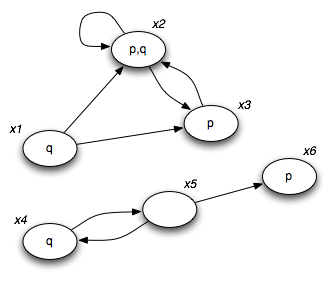
\includegraphics[width=0.65\textwidth]{./Images/Kripke01.png}
  	\caption{Beispiel einer Kripke-Struktur}
		\label{fig:mmKripke01}
	\end{center}
\end{figure}

\begin{definition}
	\label{def:reasoning}
	Sei $M = (W,R,L)$ ein Model einer Modal Logik und $\phi$ sei eine Formel nach \eqref{eqn:bnf}.
	Dann lässt sich nach folgenden Regeln schließen ob $\phi$ in einer Welt $x$ \emph{Wahr} oder \emph{Falsch} ist.
	\begin{align}
	%	\begin{split}
		x &\Vdash \top\label{eqn:semanticTrue}\\
		x &\nVdash \bot\label{eqn:semanticFalse}\\
		x &\Vdash p\text{ gdw. }p \in L(x)\label{eqn:semanticLabel}\\
		x &\Vdash \neg \phi\text{ gdw. }x \nVdash \phi\\
		x &\Vdash \phi \wedge \psi\text{ gdw. }x \Vdash \phi\text{ und } x \Vdash \psi\label{eqn:semanticAnd}\\
		x &\Vdash \phi \vee \psi\text{ gdw. }x \Vdash \phi \text{, oder } x \Vdash \psi\\
		x &\Vdash \phi \rightarrow \psi\text{ gdw. }x \Vdash \psi\text{, immer wenn gilt }x \Vdash \phi\\
		x &\Vdash \phi \leftrightarrow \psi\text{ gdw. }( x \Vdash \phi\text{ gdw. }x \Vdash \psi)\label{eqn:semanticBiconditional}\\
		x &\Vdash \Box \psi \text{ gdw. }\forall y \in W \text{ gilt } R(x,y)\text{, und } y \Vdash \psi\label{eqn:semanticBox}\\
		x &\Vdash \Diamond \psi\text{ gdw. }\exists y \in W \text{ sodass }R(x,y)\text{ und }y \Vdash \psi\label{eqn:semanticDiamond}
	%	\end{split}
	\end{align}	
\end{definition}
\cite[S.310]{huth2004logic}\\
\\
%
%
Die Formeln \eqref{eqn:semanticTrue} und \eqref{eqn:semanticFalse} besagt, dass die Werte \true und \false enthalten sind. 

Die Formel \eqref{eqn:semanticLabel} besagt, dass wir Aussagen folgern können die Teil der Wissensbasis sind.

Die Formeln \eqref{eqn:semanticAnd} bis \eqref{eqn:semanticBiconditional} sind ähnlich zu denen aus der Aussagenlogik.

Besonders zu beachten sind die Formeln \eqref{eqn:semanticBox} und \eqref{eqn:semanticDiamond}. 
\eqref{eqn:semanticBox} besagt, dass die Aussage $\Box\psi$ für eine Welt $x$ gefolgert werden kann, wenn diese in allen Welten die von $x$ aus erreichbar sind, folgerbar ist. 
Dies beinhaltet $x$ nur wenn $R(x,x)$ gilt.
Wichtig ist das die Aussage lediglich fordert, das eine Aussage in allen \emph{erreichbaren} Welten gefolgert werden kann. $x \Vdash \Box \bot$ ist also \true wenn $x$ mit keiner anderen Welt verbunden ist.

Die Formel \eqref{eqn:semanticBox} ist ähnlich, nur das sie einen Existenz-Charakter hat. 
Aus $x$ lässt sich $\Diamond \psi$ folgern, wenn es min. eine Welt gibt die von $x$ erreichbar ist, in der sich $\psi$ folgern lässt. 
Wichtig ist die Aussage \emph{es existiert} eine Welt. 
$x \Vdash \Diamond \top$ ist also \false wenn es keine Welt $x'$ gibt für die gilt $R(x,x')$.\\


\begin{figure}
	\centering
	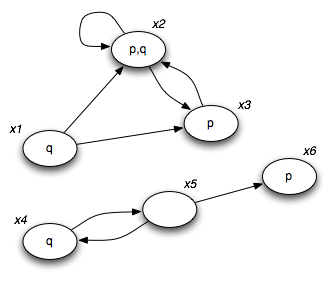
\includegraphics[height=6.5cm]{Images/Kripke01.png}
	\caption{Kripke Model Beispiel für Model Folgerungsbeispiele}
	\label{fig:Kripke01}
\end{figure}


\begin{definition}
	\label{def:model_erfuellt}
	Ein Model $\mathcal{M}$ einer Modal Logik erfüllt eine Formel $\phi$ wenn jeder Zustand im Model die Formel erfüllt.
	Wir schreiben für diesen Fall $\mathcal{M} \vDash \psi$ gdw. $\forall x \in W, x \Vdash \psi$ gilt.
\end{definition}
\cite[S.310f]{huth2004logic}
%
Anhand des Kripke Models \Abb{Kripke01} werden nun ein paar Beispielformeln diskutiert um die Definitionen zu konkretisieren:

\curr
\begin{itemize}
	\item $x_1 \vDash q$, gilt wegen $q \in L(Lx_1)$
	\item $x_1 \vDash \Diamond q$, weil es einen erreichbare Welt (hier $x_2$) $q \in L(x_2)$ gilt. Mathematisch formuliert: es gilt $R(x_1, x_2)$ und $x_2 \vDash q$
	\item $x_1 \nvDash \Box q$, weil $R(x_1,x_3)$ und $x_3 \nvDash q$. $\Box$ setzt voraus, dass \emph{alle} erreichbaren Welt die Bedingung erfüllen.
	\item $x_5 \nvDash \Box p$ und $x_5 \nvDash \Box q$ sogar $x_5 \nvDash \Box p \vee \Box q$, allerdings gilt $x_5 \vDash \Box (p \vee q)$. $x_5 \nvDash \Box p$ gilt, weil $x_4$ erreichbar ist, aber nicht $p$ enthält. $x_5 \nvDash \Box q$ gilt weil, $x_6$ erreichbar ist aber kein $q$ enthält. Damit gilt auch $x_5 \nvDash \Box p \vee \Box q$. $x_5 \vDash \Box (p \vee q)$ gilt hingegen, weil alle erreichbaren Welten $(x_5, x_6)$ entweder $p$ oder $q$ enthalten.
	\item Die Welten die $\Box p \rightarrow p$ erfüllen sind: $x_2, x_3, x_4, x_5, x_6$.
	Die Welten $x_2, x_3, x_6$ erfüllend die Formeln mit \true, weil sei $p$ enthalten und $\Box p$ gilt. Für $x_6$ gilt $\Box q$ weil es keine erreichbaren Welten hat (vgl. Formel \eqref{eqn:semanticBox} ).
	Die Welten $x_4, x_5$ erfüllen die Formel mit \false, weil sie $p$ nicht enthalten und nicht alle von ihnen erreichbaren Welten $p$ enthalten. $x_5 \nvDash \Box p$ ist der Fall, weil $x_4$ zutrifft.
\end{itemize}
%
Welten wie $x_6$ die keine Verbindungen zu anderen Welten erfordern besonderes Augenmerk.
Die Formel $x_6 \nvDash \Diamond \phi$ gilt z.B. immer, auch wenn $\phi = \top$ weil $\Diamond$ min eine verbundene Welt voraussetzt.
$x \nvDash \Diamond \top$ gilt z.B. immer wenn $x$ min. eine erreichbare Welt hat, weil $\top$ per Definition in jeder Welt erfüllt ist.
Ähnlich verhält es sich mit $x_6 \vDash \Box \phi$. Diese Aussage gilt immer egal welchen Wert $\phi$ besitzt.
Das gilt auch für die Aussage $x_6 \Vdash \Box \bot$. 
Auch wenn $\bot$ per Definition in jeder Welt \false ist, ist die Aussage $x_6 \Vdash \Box \bot$ \true, wenn es keine anderen verbundenen Welten gibt.
Es ist schlicht weg nicht möglich das Gegenteil zu beweisen, weil es keine Gegenbeispiele geben kann.
Auch wenn diese Interpretationen nicht intuitiv sind, sichern die sie die Morgen Bedingung siehe \eqref{eqn:semanticBox}



%
%
\paragraph{\formelSchemata} % (fold)
\label{par:formel_schemata}
\formelSchemata beschreiben eine generelle Form, ein Pattern, von Formeln.
Ihr \parseTree ist unvollständig, an jedem Blatt ist platz für eine weitere valide \ML Formel.
Jede Belegung eines solchen \formelSchema wird \fachwort{Instanz} genannt.
Die Anzahl der möglichen Instance ist unendlich.\\
\\
Hier ein paar Instanzen-Beispiele für das \formelSchema $\psi \rightarrow \Box \Diamond \psi$:\\
\begin{itemize}
	\item $p \rightarrow \Box \Diamond p$
	\item $q \rightarrow \Box \Diamond q$
	\item $(p \wedge r \rightarrow q) \rightarrow \Box \Diamond (p \wedge r \rightarrow q)$
\end{itemize}

% paragraph formel_schemata (end)

\textbf{Gleichheit zwischen modal logischen Formeln}
\begin{definition}
	\label{def:model_folgert}
	\begin{itemize}
		\item Eine Menge von modal logischen Formeln $\Gamma$ folgert eine modal logische Formel $\psi$, gdw. wenn für jede Welte $w$ aus jedem Model $\mathcal{M}$ gilt $x \Vdash \psi$ immer wenn gilt $x \Vdash \phi$ $\forall \phi \in \Gamma$. 
		Dies wird notiert durch $\Gamma \vDash \psi$.
		\item Wir bezeichnen zwei modal logische Formeln $\phi$ und $\psi$ als semantisch äquivalente wenn sowohl $\psi \vDash \phi$ als auch $\psi \vDash \phi$ gilt und notieren dies mit $\psi \equiv \phi$.
	\end{itemize}	
\end{definition}
\cite[S.313]{huth2004logic}


\begin{equation}
	\neg \Box \phi \equiv \Diamond \neg \phi \text{ und } \neg \Diamond \phi \equiv \Box \neg \phi
\end{equation}


\textbf{valide Formeln}
\begin{definition}
	\label{def:valide}
	Eine modal logische Formel $\psi$ wird valide genant wenn sie in jeder Welt in jedem Model \emph{Wahr} ist, also gdw. $\vDash \psi$ gilt.
\end{definition}
\cite[S.314]{huth2004logic}

Dadurch das man bestimme Formeln als valide voraussetzt, kann man eigene Logiken und damit andere modale von \true erzeugen.
Die \NML $K$ schreibt nur die Validität der Formel \KFormel vor.
Diese bewirkt, dass \todo{Wirkung eintragen}.\\
Im nächsten Kapitel werden weitere Formeln, die als valide vorausgesetzt werden können, vorgestellt und deren Auswirkungen diskutiert.







% section semantik (end)

%!TEX root = /Users/velrok/Dropbox/TheoInf Seminar/Ausarbeitung/Main.tex


\section{Attribute einer Modal-Logik} % (fold)
\label{sub:attribute_einer_modal_logik}
Die Attribute einer \ML werden dadurch bestimmt welche Formeln als valide vorausgesetzt werden.
Alle \NML setzen die Validität der Formel $K$, die Formel für die Logische Konsequentz \todo{Quelle referenzieren}, voraus.
\NNML sind nicht Teil dieser Arbeit. Der interessierte Leser sein an Priest \cite[S.75ff]{Priest:2008} verwiesen.
Will man eine eigene \ML kreieren ist es wichtig sich genaue Gedanken darüber zu machen, welcher Formeln die als valide voraussetzt, weil das die Eigenschaften der zu modellierenden Wahrheit bestimmt.
Im Folgenden wird erst das für \NML zwingend erforderliche Basisattribut $K$ vorgestellt und danach auf die anderen optionalen Eigenschaften eingegangen.
Zum Schluss werden ein paar \NML und deren Eigenschaften beschrieben und erklärt warum die gewählten Eigenschaften für die Modalität wünschenswert / wichtig / notwendig sind.\\
%
\curr



\paragraph{Das Basis Atribute $K$} % (fold)
\label{par:das_basis_atribute_k_} Die Formel $K$ \KFormel besagt, dass es nur normale Welten gibt. Das heißt die Wahrheitsmodulation $\Box$ verhält sich immer gleich im Gegensatz zu \NNML wo es \fachwort{nicht normale} Welten geben kann.
In nicht normalen Welten ist vereinfacht formuliert alles möglich und nichts notwendig.\cite[S.75]{Priest:2008}



\paragraph{Weitere Attribute} % (fold)
\label{par:weitere_attribute} 

Neben der Formel für $K$ gibt es weitere typische Formeln die, sofern sie als valide vorausgesetzt werden einer \NML gewissen Eigenschaften verleihen.


\todo{weiter Atribute diskutieren}
\textbf{einige Modal Logiken}



\begin{definition}
	Ein Modell der intuitionistischen Aussagenlogik ist ein Model \modelFormel der Logik $KT45$, sodass $R(x,y)$ immer $L(x) \subseteq L(y)$ impliziert.
	Gegeben einer modal logische Formel nach \eqref{eqn:bnf}, definieren wir $x \Vdash \psi$ wie in Definition \eqref{def:reasoning} mit Außnahme der Reglen für $\rightarrow$ und $\neg$.
	\begin{itemize}
		\item $\psi \rightarrow \phi$ definierten wir als $x \Vdash \psi \rightarrow \phi$ gdw. $\forall y R(x,y)$ auch $y \Vdash \phi$ gilt, immer wenn $y \Vdash \psi$ gilt.
		\item $\neg \psi$ definierten wir als $x \Vdash \neg \psi$ gdw. $\forall y R(x,y)$ $y \nVdash \psi$ der Fall ist.
	\end{itemize}
\end{definition}
\cite[S.328]{huth2004logic}

\begin{definition}
	Gegeben einer Menge von Formel Schemata $\mathds{L}$.
	Definieren wir $\Gamma \Vdash_\mathds{L} \psi$ als valide, wenn es einen Beweis im natürlichen Folgerungssystem für modal Logiken gibt, der um die Axiome in $\mathds{L}$ und den Annahmen in $\Gamma$ erweitert ist.
	\todo{bessere Forumlierung finden}
	\todo{natural deduction system beser übersetzen}
\end{definition}
\cite[S.330]{huth2004logic}

\begin{definition}
	\label{def:substitution}
	Sei $\mathds{L}$ eine Menge von Formel-Schemata der Modal Logik und $\Gamma \cup {\psi}$ eine Menge von modal logischen Formeln.
	
	\begin{itemize}
		\item Die Menge $\Gamma$ ist abgeschlossen gegenüber der Substitution von Instanzen gdw.  $\psi \in \Gamma$. 
		Dann gilt auch, dass jede Substitutionsinstanz von $\psi$ auch in $\Gamma$ ist.
		\item Sei $\mathds{L}_c$ die kleinste Menge die alle Instanzen von $\mathds{L}$ enthält.
		\item Aus $\Gamma$ folgt semantisch $\psi$ in $\mathds{L}$ gdw. alle Modelle, deren Frame $\mathds{L}$ erfüllt und alle Welten $x$ in diesem Modell, $x$ erfüllt $\Gamma$, gilt.
		In diesem Fall sagen wir $\Gamma \vDash_{\mathds{L}} \psi$ ist erfüllt.
	\end{itemize}
	\cite[S.326]{huth2004logic}
\end{definition}




% paragraph abgesehen_davon_gibt_es_weitere_attribute (end)
% paragraph das_basis_atribute_k_ (end)
% subsection attribute_einer_modal_logik (end)

%!TEX root = /Users/velrok/Dropbox/TheoInf Seminar/Ausarbeitung/Main.tex
\curr
\section{Ähnlichkeitstheorie} % (fold)
\label{sub:Aehnlichkeitstheorie}

Die Ähnlichkeitstheorie besagt, das sich die Eigenschaften einer Modal-Logik in der Relation der entsprechenden Kripkestrucktur widerspiegeln und vis versa. 
Dies schafft einen neuen Zugang zum Design von Modal-Logiken. 
In manchen Fällen mag es einfacher sein in den notwendigen Eigenschaften in Form von Formel-Schemata zu denken, in anderen ist es evtl. einfacher das Problem über die Relation zu verstehen. 
Im Folgenden wird gezeigt, wie die einzelnen Eigenschaften mit der Kripke-Struktur-Relation zusammen hängen.

\begin{definition}
	\label{def:frame}
	Ein Frame $F = (W,R)$ ist eine Menge von Welten $W$ und eine binäre Relation $R$ auf $W$.
\end{definition}
\cite[S.322]{huth2004logic}
\note{labeling funktion fehlt}


\begin{definition}
	\label{def:frame_erfuellt}
	Ein Frame $F$ erfüllt eine modal logische Formal $\psi$, wenn für jede \fachwort{Labelfunktion} $L: W \rightarrow P(Atome)$ und jedes $w \in W$, es der Fall ist, dass $M,w \vDash \psi$ gilt. $M$ ist das Model: $M = (W,R,L)$.
	In diesem Falle schreiben wir $\mathds{F} \vDash \psi$.
	\cite[S.322f]{huth2004logic}
\end{definition}





\todo{mehr schreiben}

% subsection Aehnlichkeitstheorie (end)

%!TEX root = /Users/velrok/Dropbox/TheoInf Seminar/Ausarbeitung/Main.tex


\section{Die Modal-Logik $KT45$ (Wissen)} % (fold)
\label{sub:the_normal_modal_logic_s5_}

Die \ML wird definiert durch eine Menge an gültigen \formelSchemata $\Menge{L}$.
Die \Tab{attributesIncludingR} zeigt einige der wichtigsten dieser \formelSchemata.

\begin{definition}
	\label{def:substitution}
	Sei $\mathds{L}$ eine Menge von Formel-Schemata der \ML und $\Gamma \cup {\psi}$ eine Menge von modal logischen Formeln.
	
	\begin{itemize}
		\item Die Menge $\Gamma$ ist abgeschlossen gegenüber der Substitution von Instanzen gdw.  $\psi \in \Gamma$. 
		Dann gilt auch, dass jede Substitutionsinstanz von $\psi$ auch in $\Gamma$ ist.
		\item Sei $\mathds{L}_c$ die kleinste Menge die alle Instanzen von $\mathds{L}$ enthält.
		\item Aus $\Gamma$ folgt semantisch $\psi$ in $\mathds{L}$ gdw. alle Modelle, deren Frame $\mathds{L}$ erfüllt und alle Welten $x$ in diesem Modell gilt, $x$ erfüllt $\Gamma$.
		In diesem Fall sagen wir $\Gamma \vDash_{\mathds{L}} \psi$ gilt.
	\end{itemize}
	\cite[S.326]{huth2004logic}
\end{definition}

Bei der \ML $KT45$ handelt es sich um eine bekannte Logik zur Modellierung von Wissen.
Sie wird in der Literatur auch mit $S$ bezeichnet.
Die Formel $\Box \phi$ bezeichnet dass ein Agent $Q$ die Tatsache $\phi$ weiß.
Die Menge der vorausgesetzten \formelSchemata ist $\Menge{L} = \{T, 4, 5\}$.\\
\textbf{T} bedeutet in diesem Zusammenhang, dass nur Dinge gewusst werden können, die auch \true sind.\\
\textbf{4} \emph{Positive Introspektion} bedeutet, dass wenn man etwas weiß, dann weiß man, dass man es weiß.
\textbf{5} \emph{Negative Introspektion} bedeutet, dass wenn man etwas nicht weiß, dann weiß man, dass man es nicht weiß.
\textbf{K} \emph{Logische Allwissenheit} bedeutet, dass dem Agenten alle möglichen Folgerungen aus seinem Wissen ebenfalls bekannt sind.

Es ist wichtig anzumerken, dass es sich hierbei um eine stark idealisierte Modellierung von Wissen handelt.
Auf menschliches Wissen treffen diese Eigenschaften \underline{nicht} zu.
Nicht einmal alle Agenten-Systeme erfüllen all diese Eigenschaften. \citeHuth{S. 326f}


\begin{fact}
	Eine Relation ist reflexiv, transitiv und euklidisch gdw. sie reflexiv, transitiv und symmetrisch ist, es sich also um eine Äquvivalenzs-Relation handelt. \citeHuth{S.327}
\end{fact}

Die \ML $KT45$ ist simpler als $K$, weil weniger sich tatsächlich unterscheidende Aussagen möglich sind.

\begin{theorem}
	Jede Folge von Modal-Operatoren und Negationen in $KT45$ ist gleichbedeutend zu einer der folgenden Kombinationen: $-$, $\Box$, $\Diamond$, $\neg$, $\neg \Box$ und $\neg \Diamond$, wobei $-$ bedeutet, dass kein Modal-Operator und keine Negation verwendet wird. \citeHuth{S. 327}
\end{theorem}


% subsection the_normal_modal_logic_s5_ (end)
\section{Intuistische \ML} % (fold)
\label{sec:intuistische_ml}

\begin{definition}
	\label{intuistischeLogiken}
	Ein Modell der intuitionistischen Aussagenlogik ist ein Model \modelFormel der Logik $KT45$, sodass $R(x,y)$ immer $L(x) \subseteq L(y)$ impliziert.
	Gegeben einer modal logische Formel nach \eqref{eqn:bnf}, definieren wir $x \Vdash \psi$ wie in Definition \eqref{def:reasoning} mit Außnahme der Reglen für $\rightarrow$ und $\neg$.
	\begin{itemize}
		\item $\psi \rightarrow \phi$ definierten wir als $x \Vdash \psi \rightarrow \phi$ gdw. $\forall y R(x,y)$ auch $y \Vdash \phi$ gilt, immer wenn $y \Vdash \psi$ gilt.
		\item $\neg \psi$ definierten wir als $x \Vdash \neg \psi$ gdw. $\forall y R(x,y)$ $y \nVdash \psi$ der Fall ist.
	\end{itemize}
\end{definition}
\cite[S.328]{huth2004logic}


% section intuistische_ml (end)
%!TEX root = /Users/velrok/Dropbox/TheoInf Seminar/Ausarbeitung/Main.tex

\section{\ND} % (fold)
\label{sub:natuerliche_folgerung}
Natürliche Deduktion ist ein Kalkül um aus einer Menge von aussagen-logischen Formeln andere Formeln abzuleiten.
Dazu gibt es eine Menge von Regeln die hier aufgelistet aber nicht im Detail erklärt werden.
Eine gute Erklärung der Grundlagen des Systems findet sich in Huth \cite[Kapitel 1.2 (natural deduction)]{huth2004logic} in englischer Sprache.\\
\\
Das System wurde für aussagen-logische Formeln entwickelt. Es lässt sich jedoch erweitern um in der \ML Beweise der Form $\Gamma \vDash_\Menge{L} \psi$ führen zu können.\\

\paragraph{\ND \AL} % (fold)
\label{par:natuerliche_deduktion_aussagenlogick}
Die \ND erlaubt das formelle folgern von Aussagen anhand eines festen Regelsatzes.
Die \Eq{iConjunction} zeigt eine solche Regel.

\begin{equation}
	\label{eq:iConjunction}
%	\boxed{
%	\begin{array}{rcl}
		\frac{\phi \qquad \psi}{\phi \wedge \psi} \wedge i
%	\end{array}
%	}
\end{equation}


Jede Regel hat drei Bestandteile:
\begin{itemize}
	\item Die \underline{Voraussetzung} befindet sich über dem Bruchstrich.
	\item Die \underline{Folgerung} lässt sich unter dem Bruchstrich finden.
	\item Der \underline{Name} oder der Bezeichner wird rechts an die Gleichung angehangen.
\end{itemize}
Es lässt sich dabei zwischen Einführungs- (gekenzeichnet durch ein $i$) und Eliminierungsregeln (gekenzeichnet durch ein $e$) unterscheiden.
Die \Eq{iConjunction} ist also ein Beispiel für eine Einführungsregel.
Sie führt die Konjunktion $\phi \wedge \psi$ ein.\\
\\
Manchmal ist es notwendig Formeln temporär als gegeben anzunehmen um einen allgemein gültigen Schluss ziehen zu können. Huth \cite[S.11]{huth2004logic} erklärt dies sehr verständlich.\\
Die Gültigkeit einer solchen temporären Annahme wird durch eine Box um den Teil des entsprechenden Beweises gekennzeichnet.\\
\begin{equation}
	\label{eq:iImplication}
	\frac{
		\boxed{
			\begin{array}{c}
					\phi\\
					\vdots\\
					\psi\\
			\end{array}
		}
	}
	{\phi \rightarrow \psi} \rightarrow i
\end{equation}
Ein Box kann selbst wieder weitere Boxen enthalten.
Ein Box kann alle Formeln verwenden die über Annahmen in dieser Box erzeugt wurden und die vor der Box bereits verfügbar waren.
Annahmen dürfen eine Box nicht verlassen. Lediglich die Folgerungen können danach verwendet werden.

\begin{equation}
	\boxed{\begin{array}{c}
		A\\
		\vdots\\
		a_1\\
		\boxed{\begin{array}{c}
		B_1\\
		\vdots
		\end{array}}\\
		f_1\\
		\vdots\\
		a_2\\
		\boxed{\begin{array}{c}
		B_2\\
		b_{2_1}\\
		\boxed{\begin{array}{c}
		C\\
		\vdots\\
		\end{array}}\\
		\vdots\\
		\end{array}}
	\end{array}}
\end{equation}

Die Sichtbarkeit von Formeln ist sehr wichtig, deswegen hier noch ein Beispiel um dies zu verdeutlichen.\\
Innerhalb der Box $B_1$ sind alle Formeln der Box $A$ sichtbar die bis dahin deklariert wurden, weil $B_1$ eine Box innerhalb der Box $A$ ist. In diesem Falle ist das die Variable $a_1$.\\
Innerhalb der Box $B_2$ sind ebenfalls alle Formeln aus $A$ verfügbar ($a_1$ $a_2$ $f_1$), allerdings \emph{nicht} die aus $B_1$, weil $B_2$ nur innerhalb von $A$ liegt, nicht jedoch innerhalb von $B_1$.
Weil die Folgerung aus $B_1$ nun teil von $A$ ist kann $B_2$ diese ebenfalls verwenden.\\
Die Box $C$ liegt innerhalb von $A$ und $B_2$ und kann damit alle Formeln von $A$ und $B_2$ verwenden ($a_1$ $f_1$ $a_2$ $b_{2_1}$).

\\



% paragraph natürliche_deduction_aussagenlogick (end)

\paragraph{\ND \ML} % (fold)
\label{par:natuerliche_deduktion_ml}

% paragraph natürliche_deduktion_ml (end)

% subsection natürliche_folgerung (end)

% section basic_modal_logic (end)

%!TEX root = /Users/velrok/Dropbox/TheoInf Seminar/Ausarbeitung/Main.tex


\chapter{Multi-Modal-Logic} % (fold)
\label{sec:multi_modal_logic}
\MML sind \NML die mehr als eine Modularität der Wahrheit enthalten.
Ein Beispiel dafür sind Multi-Agent-Systeme. 
In einem solchen System, kann ein Agent nicht nur Folgerungen auf Basis seines Wissens, sonder auch auf Basis des Wissen über das Wissen der anderen anstellen. Also Aussagen der Art: Weil \emph{ich} weis das \emph{er} \textbf{A} weis kann ich \textbf{B} folgern.
Konkret wird dieses Kapitel die Logik $KT45^n$, den allgemeinen Fall der Wissenslogik $KT45$, anhand der klassischen Logik Rätsel \emph{Wise-Men} und \emph{Muddy-Children} darstellen.

%!TEX root = /Users/velrok/Dropbox/TheoInf Seminar/Ausarbeitung/Main.tex


\section{Das Wise-Men Rätsel} % (fold)
\label{sub:das_wise_men_raetsel}

Das \emph{Wise-Men-Puzzle} ist ein klassisches Beispiel dafür wie ein Agent aufgrund von Allgemeinwissen und das Wissen über das Wissen oder Unwissen andere Folgerungen ziehen kann.

\begin{puzzle}
	\label{puz:wiseMen}
	Es gibt 3 weise Männer.
	Es gehört zum Allgemeinwissen - etwas das jeder weiß, und jeder weiß, dass es jeder weiß, was wiederum jeder weiß usw. -, dass es 3 rote und 2 weiße Hüte gibt.
	Der König setzt jedem der weisen Männer einen Hut auf, sodass jeder nur die Hüter der anderen, nicht jedoch seinen eigenen sehen kann.
	Danach fragt er der Reihe nach jeden ob er weiß welche Farbe sein Hut hat.
	Gehen wir davon aus, dass sowohl der Erste als auch der Zweite es nicht weiß, dann folgt daraus, dass der Dritte Wissen muss welche Farbe sein Hut hat.
	\\
	Warum?\\
	Welche Farbe hat sein Hut?
\end{puzzle}
%
%
Das Rätsel setzt folgendes Vorraus:
\begin{itemize}
	\item Alle Beteiligten sind ehrlich
	\item Alle Beteiligten sind schlau (übersehen keine Folgerungen)
	\item Alle Beteiligten wissen das die anderen schlau sind
	\item Alle Beteiligten besitzen dasselbe Allgemeinwissen
\end{itemize}
%
%
Im folgenden wird das Rätsel umgangssprachlich und durch Überlegungen gelöst. In \Abs{sub:the_modal_logic_kt45_n_} wird das Rätsel in der \MML $KT45^n$ formalisiert und formal gefolgert.\\
\\
Beginnen wir damit alle möglichen Kombinationen zu notieren:\\
%
\begin{tabular}{ccc}
\texttt{R R R} &   & \texttt{W R R}\\
\texttt{R R W} &   & \texttt{W R W}\\
\texttt{R W R} &   & \texttt{W W R}\\
\texttt{R W W} &   &   \\
\end{tabular}
%
Wobei die Notation \texttt{R R W} bezeichnet, dass der Erste und Zweite einen roten und der Dritte einen weißen Hut tragen.
Der Fall \texttt{W W W} kann nicht auftreten, weil es keine 3 weißen Hüte gibt.\\
Betrachtet man das Rätsel mal aus der Perspektive des 2. und 3. Weisen. 
Nach der negativ Aussage vom Ersten kann der Zweite folgern, dass \texttt{R W W}, nicht der Fall ist, sonst wüste der 1. das er einen roten Hut trägt. 
Mit der selben Argumentation kann der 3. den Fall \texttt{W R W} ausschließen. 
Damit bleiben folgende Kombinationen:\\
\begin{tabular}{ccc}
\texttt{R R R} &   & \texttt{W R R}\\
\texttt{R R W} &   & \sout{\texttt{W R W}}\\
\texttt{R W R} &   & \texttt{W W R}\\
\sout{\texttt{R W W}} &   &   \\
\end{tabular}
%
Der 3. kann außerdem den Fall \texttt{R R W} ausschließen, denn wäre dies der Fall gewesen hätte der 2. gefolgert, dass es einer der beiden Kombinationen \texttt{R R W} oder \texttt{R W W} zutreffen muss.
Der Fall \texttt{R W W} konnte aber schon durch die Aussage des Ersten ausgeschlossen werden.
Wäre also \texttt{R R W} der Fall gewesen, so hätte der Zwei gewusst, dass er einen roten trägt. Da er das aber nicht sagt, kann dieser Fall ausgeschlossen werden.
Damit bleiben übrig:\\
%
\begin{tabular}{ccc}
\texttt{R R R} &   & \texttt{W R R}\\
\sout{\texttt{R R W}} &   & \sout{\texttt{W R W}}\\
\texttt{R W R} &   & \texttt{W W R}\\
\sout{\texttt{R W W}} &   &   \\
\end{tabular}
Wie man sehen kann, trägt der 3. in jedem der Fällt einen roten Hut.
Deswegen kann er folgern, dass er einen roten Hut aufhaben muss, weil sonst einer der anderen anders geantwortet hätte.\\
Das zeigt, warum es notwendig ist, dass alle Beteiligten schlau sind, nichts übersehen, nicht lügen und all dies zum Allgemeinwissen der Beteiligten zählt.




% subsection das_wise_men_ (end)

%!TEX root = /Users/velrok/Dropbox/TheoInf Seminar/Ausarbeitung/Main.tex


\subsection{Das Muddy-Children Rätsel} % (fold)
\label{sub:das_muddy_children_raetsel}

% section das_muddy_children_rätsel (end)

%!TEX root = /Users/velrok/Dropbox/TheoInf Seminar/Ausarbeitung/Main.tex

\section{Die Modal-Logik $KT45^n$ (Multi-Agent-Wissen)} % (fold)
\label{sub:the_modal_logic_kt45_n_}

Die \MML $Kt45^n$ ist eine Verallgemeinerung der \ML $KT45$, in der Hinsicht als dass es mehrerer $\Box$ ähnliche Operatoren gibt.
Jeder Agent einer Menge \AgentSetDef hat seine eigene Relation $R_i$ auf $W$.
Der Operator eines Agenten $i$ wird notiert als $K_i$ mit $K$ für \emph{Knowlage} (Wissen).
Wir verwenden weiterhin $p,q,r$ für atomare Terme.
Die $K_ip$ bedeutet das Agent $i$ die Tatsache $p$ weis.
Hier nun eine komplexeres Beispiel einer Formel in $KT45^n$ : $K_1p \wedge K_1 \neg K_2 K_1 p$.
Sie besagt: Agent 1 weis $p$, außerdem weis Agent 1, das Agent 2 nicht weis, dass er $p$ weis.
Mit $G$ beschreiben wir eine Gruppe von Agenten $G= \{1,2,3,\dots,n\}$.
Will man nun Aussagen das eine Gruppe $G$ von Agenten einen Umstand $p$ weis : $K_1 p \wedge K_2 p \wedge \dots K_n p$ benutzt man dafür die Formulierung $E_G p$.
Es gelden die selben Bindungsstärke der Operatoren wie in der Auflistung \Ref{bindungsstaerke}.
Wobei $K_i$ wie der $\Box$-Operator behandelt wird.
\citeHuth{S.335ff}


Bei erster Betrachtung mag man annehmen, dass eine Tatsache $\phi$ nicht bekannter sein kann als $E_G \phi$.
$E_G E_G \phi$ stellt jedoch mehr Wissen dar als $E_G \phi$, denn es besagt nicht nur das jeder etwas weis, sondern auch das jeder weis, dass es jeder weis.
Genauso stellt $E_G E_G E_G \phi$ wiederum noch mehr Wissen dar, denn jeder Weis, dass alle etwas wissen und \emph{das} ist wiederum bekannt.
Dies lässt sich ins unendliche fortsetzen $E_G E_G \dots \phi$.
Da es aber nur möglich ist finite Aussagen zu machen, für diesen Umstand des Allgemeinwissens ein extra Operator $C_G$ eingeführt und über seine Semantik definiert.
Wir bezeichnen als mit $C_G$ das Allgemeinwissen innerhalb einer Gruppe $G$.
Mit $D_G$ wollen wir verteiltes Wissen beschreiben.
Verteiltes wissen ist dem Einzelnen evtl. nicht bekannt, kann jedoch gefolgert werden, sobald alle Beteiligten der Gruppe ihr Wissen vereinen.
Die Buchstaben $C$ und $D$ stammen aus dem Englischen für common-knowlage und distributed-knowlage.

\textbf{multi agent systeme}
\begin{definition}
	\label{def:bnf_kt45n}
	Eine Formel $\psi$ der multi modal Logik $KT45^n$ ist definiert durch folgende Grammatik:
	\begin{equation}
		\label{eqn:bnf_kt45n}
		\phi ::= \bot|\top|p|(\neg\phi)|(\phi\wedge\phi)|(\phi\vee\phi)|(\phi\rightarrow\phi)|
		(\phi\leftrightarrow\phi)|(K_i\psi)|(E_G\psi)|(C_G\psi)|(D_G\psi)
	\end{equation}
	wobei $p$ irgendeine atomare Formel ist und $i \in \Fancy{A}$ sowie $G \subseteq \Fancy{A}$ gilt.
	$E_\Fancy{A}, C_\Fancy{A}, D_\Fancy{A}$ werden zur Einfachheit ohne den extra Index geschrieben $E,C,D$.
	\citeHuth{S.335f}
\end{definition}


Vergleicht man diese Definition mit der von 
\Def{syntax} so stellt man fest, dass anstelle des 
$\Box$ Operator nun eine Vielzahl von Operatoren gibt: 
$K_i, E_G, C_G, D_G$ für alle $ G \subseteq \Fancy{A}$.
Im Folgenden wird gezeigt das sich diese Operatoren $\Box$ ähnlich verhalten.
Es gibt kein explizites Analogon zu $\Diamond$.
Es ist aber entsprechend gleichbedeutend mit $\neg K_i \neg, \neg E_G \neg, \neg C_G \neg, \neg D_G \neg$.


\begin{definition}
	Ein Model \MMModelDef der \MML $KT45^n$ mit der Menge $\Fancy{A}$ von $n$ Agenten wird beschrieben durch drei Dinge:
	\begin{enumerate}
		\item einer Menge $W$ von möglichen Welten
		\item für jedes $i \in \Fancy{A}$, der Gleichheitsrelation $R_i$ auf $W$ $R_i \subseteq W \times W)$ auch Erreichbarkeitsrealtion gennant und
		\item der Labeling-Funktion $L: W \rightarrow \Fancy{P}(Atome)$
	\end{enumerate}
	\cite[S.336f]{huth2004logic}
\end{definition}

Vergleicht man diese Definition mit der \Def{model}, aus der \ML so lässt sich folgendes feststellen.
Es sind nur mehrere Relationen $R_i$, eine für jeden Agenten $i$ definiert.
Außerdem wird vorausgesetzt, dass $R$ eine Gleichheitsrelation ist, also reflexiv und symmetrisch.\\
Dieser Umstand wird bei der graphischen Darstellung von $KT45^n$ Modellen ausgenutzt.
So sind die Kanten mit den Relationen beschriftet für die sie gelten, außerdem gibt es keine Notwendigkeit für Pfeile, weil eine Verbindung durch die Symmetrie-Eigenschaft immer in beide Richtungen besteht.
Streng genommen müsste auch jede Welt, aufgrund der Transitivität, eine Verbindung auf sich selbst haben, die in jeder Relation definiert ist.
Weil dieser Umstand stand aber für alle Welten außnahmslos gilt, wird zugunsten der Übersichtlichkeit auf die Verbindungen verzichtet. \todo{Abbildung verlinken}

\todo{Bsp: grphic aus huth S. 336 erstellen}



\begin{definition}
		Gegeben ein Model $\mathds{M} = (W,(R_i)_{i \in \mathds{A}}, L)$ der $KT45^n$ und eine Welt $w \in W$, so definieren $\psi$ als \emph{Wahr} durch die Erfüllung der Relation $x \vDash \psi$ durch folgende Regeln:
		\begin{align}
			x &\Vdash p\text{ gdw. }p \in L(x)\\
			x &\Vdash \neg \phi\text{ gdw. }x \nVdash \phi\\
			%
			x &\Vdash \phi \wedge \psi\text{ gdw. }x \Vdash \phi\text{ und } x \Vdash \psi\\
			x &\Vdash \phi \vee \psi\text{ gdw. }x \Vdash \phi \text{, oder } x \Vdash \psi\\
			%
			x &\Vdash \phi \rightarrow \psi\text{ gdw. }x \Vdash \psi\text{, immer wenn gilt }x \Vdash \phi\\
			%
			x &\Vdash K_i\psi \text{ gdw. } \forall y \in W, R_i(x,y) \text{, } y \Vdash \psi \text{ impliziert}\\
			x &\Vdash E_G\psi \text{ gdw. } \forall i \in G, x \Vdash K_i\psi\\
			x &\Vdash C_G\psi \text{ gdw. } \forall k \geq 1 \text{, und es gilt } x \Vdash E^k_G\psi \text{.} \text{Wobei } E^k_G \text{ meint } E_{G}E_{G}\dots E_{G} \text{ k-mal.}\\
			x &\Vdash D_G\psi \text{ gdw. } \forall y \in W, y \Vdash \psi \text{gilt, immer wenn auch } R_i(x,y), \forall i \in G \text{gilt.}\\
		\end{align}
		\cite[S.337]{huth2004logic}
\end{definition}

Wir wollen wieder diese Definition der \MML mit ihrem Analogon in der \ML (\Def{reasoning}) vergleichen.
Die typischen Boolean Operatoren sind identisch definiert.
Alle $K_i$ verhalten sich wie der $\Box$ Operator, nur jeweils bezogen auf ihre Relation $R_i$.
$E_G$ ist auf Basis von $K$ definiert und $C_G$ wiederum auf Basis von $E_G$.\\
Es gibt keien Definition für $\Diamond$ weil dies über $\neg K \neg$ ausgedrückt werden kann.

Viele der festgestellen Eingenschaften der \ML gelten auch in der \MML nur jeweils mit Bezug auf die entsprechende Relation $R_i$:
\begin{enumerate}
	\item Ein \textbf{Frame} \MMFrameDef besteht aus einer Menge von Welten $W$ und einer Gleichheitsrelation $R_i$ für jedes $i \in \Fancy{A}$.
	\item Ein Frame \MMFrameDef erfüllt eine Formel $\phi$ gdw. für jede Labeling-Funktion \LabelFuncDef in jeder Welt $w \in W$, $\Fancy{M}, w \vDash \phi$ gilt, mit \MMModelDef. Dann schreiben wir $\Fancy{F} \vDash \phi$.
\end{enumerate}

Das \Theo{gErreichbarkeit} ist nützlich wenn es um die Beantwortung von Formel geht, die $E$ oder $C$ enthalten.
Wir wollen nun den Begriff der G-Erreichbarkeit erklären.
Seit \MMModelDef ein Model für $KT45^n$ und $x,y \in W$.
Wir nennen $y$ G-erreichbar in $k$ Schritten von $x$ wenn es $w_1, w_2, \dots, w_{k-1} \in W$ und $i_1, i_2, \dots, i_k$ in $G$ gibt, sodass 

\begin{equation*}
	x R_{i_1} w_1 R_{i_2} w_2 \dots R_{i_{k-1}} w_{k-1} R_{i_k} y
\end{equation*}

gilt.
Die Formulierung meint $R_{i_1}(x,w_1)m, R_{i_2}(w_1,w_2), \dots, R_{i_k}(w_k,w_y)$.
Eine Welt $y$ wird einfach nur G-erreichbar von $x$ genannt, wenn diese durch eine feste Anzahl an Schritten $k$ von $x$ G-erreichbar in $k$ Schritten ist.

\begin{theorem}
	\label{theo:gErreichbarkeit}
	\begin{enumerate}
		\item $x \Vdash E_{G}^{k} \phi$, gdw. für alle $y$, die in $k$ Schritten von $x$ G-erreichbar sind, $y \Vdash \phi$ gilt.
		\item $x \Vdash C_{G} \phi$, gdw. für alle $y$, die von $x$ G-erreichbar sind, $y \Vdash \phi$ gilt.
	\end{enumerate}
\end{theorem}

\note{Beweis führen?}


\paragraph{Valide Formeln in $KT45^n$}
\label{par:valid_formulas_in_kt45n}
Das Schema $K$ gilt für alle Operatoren.
Alle Ebenen des Wissens sind also abgeschlossen gegenüber der logischen Konsequentz.
Wenn z.B. eine Zusammenhang $\phi$ Allgemeinwissen ist dann sind auch alle logischen Folgerungen daraus wieder Teil des Allgemeinwissens.\\
Die Operatoren $E,C,D$ sind boxähnlich weil sie Universallquantoren über die Relationen $R_{E_G}, R_{D_G}, R_{C_G}$ sind.


\begin{align}
	R_{E_G}(x,y) &\text{ gdw. } R_i(x,y) \text{ für einige } i \in G\\
	R_{D_G}(x,y) &\text{ gdw. } R_i(x,y) \text{ für alle } i \in G\\
	R_{C_G}(x,y) &\text{ gdw. } R_{E_G}^k(x,y) \text{ für jedes } k \geq 1
\end{align}


Daraus folgt, dass $E_G, D_G, C_G$ das Schema $K$ im Bezug auf $R_{E_G}, R_{D_G}, R_{C_G}$ erfüllen.
Was ist mit den anderen Schemata $T,4,5$?\\
Da $R_i$ eine Gleichheitsrelation ist folgt nach \Theo{aehnlichkeitstheorie} und  \Tab{attributesIncludingR} das für jedes $K_i$ gilt:
\begin{itemize}
	\item $\Four{K_i}{\phi}$ \emph{positive Introspektion}
	\item $\Five{K_i}{\phi}$ \emph{negative Introspektion}
	\item $\Truth{K_i}{\phi}$ \emph{Wahrheit}
\end{itemize}

$R_{D_G}$ erfüllt die die Schemata $T,4,5$, weil sie ebenfalls eine Gleichheitsrelation ist.
Die Schemata gelten aber nicht automatisch für $E_G$ und $E_C$.
$\Four{E_G}{\phi}$ gilt z.B. nicht sonst wäre Allgemeinwissen lediglich, das was jeder weiß.
$\Five{E_G}{\phi}$ gilt ebenfalls nicht.\\
Die Ursache für diese Sachverhalte ist die Tatsache, dass $R_{E_G}$ ist nicht notwendigerweise eine Gleichheitsrelation ist, obwohl dies für jedes $R_i$ gilt.\\
$\Truth{E_G}{\phi}$ ist hingegen der Fall, weil $R_{E_G}$ reflexiv ist.
Für den Fall $G \neq \emptyset$ ist $E_G \phi$ immer leer, auch wenn $\phi = \bot$, sprich $E_G \bot \rightarrow \emptyset$. \todo{kann man das so schreiben?}\\
$R_{C_{G}}$ ist eine Gleichheitsrelation, daraus folgt, dass $T,4,5$ gelten, wobei 5 $G \neq \emptyset$ fordert.





\subsection{\ND in $KT45^n$}
Die \ND von $KT45$ wird erweitert um neue Arten von blauen Boxen.
Jeweils eine für jeder der entsprechenden Operatoren.
Der Operator D wird hier nicht behandelt.\\
Wie in \Abs{par:valid_formulas_in_kt45n} gesehen könne die Axiome T 4 5 für jedes $K_i$ eingesetzte werden. 4 und 5 können hingegen für $C_G$ aber nicht für $E_G$ eigenutzt.\\
Die Regeln CE und CK sind genau genommen eine Menge von Regeln für jede Wahl eines bestimmten $k$, der Einfachheit halber werden sie aber nur mit CE und CK bezeichnet.
$EK_i$ verhält sich wie eine generelle \emph{und}-Elimination und $KE$ wie eine generelle \emph{und}-Einführung.\\
Wie auch bei den Regeln zur KT45 kann man sich die Regeln K4, K5, C4 und C5 als eine Art Striktheitsentschärfung für das Importieren und Exportieren von Formeln in bestimme Boxen vorstellen.\\
Weil K4 es erlaubt um jedes $K_i$ ein weiters $K_i$ zu ergänzen erlaubt es effektiv das unveränderte Importieren von $K_i \phi$ Formeln in $K_i$ Boxen.
Ähnliches gilt für C5 das es uns erlaubt $\neg C_G$ Formeln in $C_G$ Boxen zu importieren.\\
Das Öffnen einer Box kann man sich intuitiv als das folgern auf Basis des Wissens des entsprechenden Agenten vorstellen.
Unter dieser Betrachtung ist es ebenfalls intuitiv einleuchtend, dass eine Tatsache $\phi$ nicht einfach in eine Box gebracht werden kann, denn die existent der Tatsache bedeutet nicht gleichzeitig, dass der entsprechende Agent diese auch weis.\\
Wir erinnern uns, dass ein Agent nicht falsches wissen kann.
Daher gilt besondere Sorgfalt mit der Regel $\neg i$.
Sie darf nicht angewendet werden, wenn eine der verwendeten Annahmen außerhalb der Box existiert.\\
$C\phi$ ist besonders mächtig, weil es erlaubt die Formel $\phi$ in jeder Box zu verwenden unabhängig von dessen Schachtelungstiefe.
Die Regel $E^k \phi$ hingegen erlaub die Verwendung von $\phi$ nur in Boxen der Schachtelungstiefe $\leq k$.\citeHuth{S.339ff}





\subsection{Formalisierung des Wise Men Rätsels in $KT45^n$}
Da wir nun eine Definition der Logik $KT45^n$ könnnen wir das Wise Men Rätsel darin formulieren und lösen.\\
Zur Erinnerung: Der König setzt jeder der drei weisen Männen einen Hut auf, sodass jeder die Hüte der anderen nicht jedoch seinen eigenen sehen kann.
Es ist allgemein bekannt das es nur 3 rote und 2 weiße Hüte gibt.
Der König fragt nun jeden der Männer der reihe nach welche Farbe der Hut hat, den der Man trägt.
Wir gehen davon aus, das sowohl der erste als auch der zwei weise Mann die Aussage machen, dass sie es nicht wissen.
Es soll nun mithilfe der $KT45^n$ formal gezeigt, dass der dritte Mann dann zwangsläufig weiß, dass er einen roten Hut trägt.

Im Folgenden wird $p_i$ notieren, dass der Mann $i$ einen roten Hut auf hat und 
$\neg p_i$, dass der Mann $i$ einen weißen Hut trägt.

Die Menge $\Gamma$ enthält Formeln, die das Allgemeinwissen in $KT45^n$ beschreiben:
\begin{subequations}
	\begin{align}
		\{&C(p_1 \vee p_2 \vee p_3) \label{eq:min_ein_roter_hut}\\
		\label{eq:zweiter_kennt_farbe_von_erster}
		&C(p_1 \rightarrow K_2 p_1), C(\neg p_1 \rightarrow K_2 \neg p_1),\\
		&C(p_1 \rightarrow K_3 p_1), C(\neg p_1 \rightarrow K_3 \neg p_1),\\
		&C(p_2 \rightarrow K_1 p_2), C(\neg p_2 \rightarrow K_1 \neg p_2),\\
		&C(p_2 \rightarrow K_3 p_2), C(\neg p_2 \rightarrow K_3 \neg p_2),\\
		&C(p_3 \rightarrow K_1 p_3), C(\neg p_3 \rightarrow K_1 \neg p_3),\\
		\label{eq:zweiter_kennt_farbe_von_letzter}
		&C(p_3 \rightarrow K_2 p_3), C(\neg p_3 \rightarrow K_2 \neg p_3)\}
	\end{align}
\end{subequations}

\Eq{min_ein_roter_hut} beschreibt den Umstand, dass mindestens einer der Männer einen roten Hut tragen muss und damit auch das es nicht mehr als zwei weiße geben kann.
Die \Eq{zweiter_kennt_farbe_von_erster} bis \Eq{zweiter_kennt_farbe_von_letzter} beschreiben, dass jeder die Hutfarbe des anderen weiß, jedoch nicht seine eigenen und das dies allgemein bekannt ist.
Es ist zu beachten, dass jeweils der positiv wie der negativ Fall festgehalten wird.

Die Aussage des ersten Mannes, dass er nicht weis welche Farbe sein Hut hat lässt sich wie folgt formalisieren:
\begin{equation*}
	C(\neg K_1 p_1 \wedge \neg K_1 \neg p_1)
\end{equation*}

entsprechend die Aussage des zweiten Mannes:
\begin{equation*}
	C(\neg K_2 p_2 \wedge \neg K_2 \neg p_2)
\end{equation*}

Ein naiver Ansatz das Rätsel zu lösen könnte so aussehen:

\begin{equation}
	\Gamma, C(\neg K_1 p_1 \wedge \neg K_1 \neg p_1), C(\neg K_2 p_2 \wedge \neg K_2 \neg p_2) \Vdash K_3 p_3
\end{equation}

Auch wenn $KT45$ ist eine komplexe Logik, reicht jedoch noch nicht aus, um das Beispiel in einem Schritt erklären zu können.
Es fehlt der temporale (zeitliche) Aspekt.
$C \neg K_1 p_1$ mag z.B. wahr sein muss es aber nicht bleiben.
Nach der Aussage des Erste ist z.B. $C p_1$ bekannt und $C \neg K_1 p_1$ damit hinfällig.

Wissen hat, in unserem idealisierten System, die Eigenschaft sich anzuhäufen und bestehen zu bleiben. 
\emph{Unwissenheit hat diese Eigenschaften nicht.}
Negative Wissensaussagen der form $\neg K \phi$ können also im zeitlichen Verlauf ihre Gültigkeit verlieren.
Erneut: $KT45^n$ kennt keine zeitlichen Zusammenhänge.

Um den Beweis des wise men Rätsels zu führen, der einen zeitlichen aspekt fordert, werden wir uns durch Schrittweise beweisen behelfen indem wir jeweils den Wissensstand vor einer Ankündigung betrachten.
Die Lösung des wise men Rätsels benötigt folglich zwei Schritte.

Informel konnte die Kombination RWW nach der ersten Ankündigung ausgeschlossen werden.
Damit wird also $p_1 \vee p_2 \vee p_3$ zu $p_2 \vee p_3$.\\
Im ersten Schritt soll genau dies nun aus dem anfänglichen Wissen gefolgert werden:
$\Gamma, C(\neg K_1 p_1 \wedge \neg K_1 \neg p_1), \Vdash C(p_2 \vee p_3)$
weil $p_2 \vee p_3$ eine positive Formulierung ist, bleibt sie auch in späteren Schnitten gültig.\\
Schritt zwei kann nun das in Schritt~1 gefolgerte Wissen nutzen um die Aussage das der dritte Mann weis, dass er einen roten Hut trägt zu folgern:
$\Gamma, C(p_2 \vee p_3), C(\neg K_1 p_1 \wedge \neg K_1 \neg p_1), \Vdash K_3 p_3$

Bei dieser Vorgehensweise handelt es sich um eine schwierige Methode, weil für jeden Schritt \emph{positives} Wissen gefunden werden muss, dass zusätzlich auch noch zielführend ist für den eigentlichen zu beweisenden Schluss.

\todo{kompletten Beweis aufführen}
\todo{kompletten Beweis diskutieren}








% subsection the_model_logic_kt45_n_ (end)


% section normal_modal_logic (end)
%!TEX root = /Users/velrok/Dropbox/TheoInf Seminar/Ausarbeitung/Main.tex

\chapter{Zusammenfassung} % (fold)
\label{sec:zusammenfassung}

Die \ML beschreibt eine Modalitäten von Wahrheit,
als Beispiel wurden Notwendigkeit und Wissen aufgeführt.
Die Notwendigkeit wird in der \ML mit dem Symbol $\Box$ und die Möglichkeit mit $\Diamon$ notiert.\\
Dabei kann eine \ML verschiedene Attribute besitzen.
Die Attribute $K, T, 4$ und $5$ wurden besondern ausführlich behandelt u.a. weil sie für die Modalität Wissen, auf der der Fokus der Arbeit liegt, wichtig sind.\\
\ML werden durch den \emph{possible world} Ansatz von Kripke modelliert.
Unter Verwendung von Kripke Strukturen ergeben sich Graphen in eine Welt mit anderen möglichen Welten durch die $R$ Relation verbunden werden.\\
Die Ähnlichkeittheorie belegt einen mathematischen Zusammenhang zwischen der Attributen einer \ML und den Eigenschaften der entsprechenden Kripke Relation $R$.\\
Als ein Beispiel für eine \ML wurde die Logik $KT45$ für Wissen genauer untersucht und beschrieben.\\
\MML unterscheiden sich von \ML durch ihre Vielzahl an $\Box$ Operatoren.
Ein Beispiel dafür war die \MML $KT45^n$.
Anhand des Beispiels \emph{wise men} wurde gezeigt, wie ein umgangssprachlich formuliertes Problem formalisiert und formal gefolgert werden kann.\\
Dafür wurde die \ND eingesetzt.
Die \ND ist ein Rechensystem für \AL, \ML und \MML Logik, mit einem jeweils angepassten Regelsatz für die spezielle Logik in der gearbeitet wird.
Attribute wie $K, T, 4$ und $5$ haben dabei direkte Auswirkungen auf diesen Regelsatz.


% section zusammenfassung (end)




%Zitate/Referenzen einf\UTF{00FC}gen
\begin{small}
	\renewcommand{\baselinestretch}{0.9}\normalsize
	%\bibliographystyle{IEEE}
	\bibliographystyle{alpha}
	\bibliography{sources}
	%\nocite{*}
\end{small}

\renewcommand{\baselinestretch}{1.1}\normalsize
%!TEX root = /Users/velrok/Dropbox/TheoInf Seminar/Ausarbeitung/Main.tex
\appendix



\chapter{Regeln der \ND} % (fold)
\label{cha:regeln_der_nd}

\todo{Hier Regeln übernehmen. Huth S. 27}

\newcommand{\wedgeI}{
	\frac{\phi \qquad \psi}
	{\phi \wedge \psi}
	\wedge i
}

\newcommand{\wedgeE}{
	asdf
}


\begin{center}
	\begin{tabular}{c|cc}
	  & einführend & eliminierend\\
	\hline
	\hline
	$\wedge$ 			& $\wedgeI$ & $\wedgeE$\\
	$\vee$ 				& r3c2 & r3c3\\
	$\rightarrow$ & r4c2 & r4c3\\
	$\neg$ 				& r5c2 & r5c3\\
	$\bot$ 				& r6c2 & r6c3\\
	$\neg \neg$ 	& r7c2 & r7c3\\
	$\Box$ 				& r8c2 & r8c3\\
	\end{tabular}
\end{center}

% chapter appendix (end)

\end{document}
